\section{Lazy Training in NNPDF}
\label{sec:LazyTraining}

In the previous section we presented an empirical study of the training dynamics
through the lens of the NTK. We observed that the NTK is able to capture the
main features of the training process, and that its time evolution is
characterised by a rapid initial transient, followed by a slower evolution
during the rest of the training. We now turn our attention on this last stage of
the training, where the NTK has stabilised and becomes approximately constant.
In doing so, we will build upon the results presented in
Refs.~\cite{jacot2018neural,lee2019wide} and extend them to the case of NNPDF.
In the following, we derive the analytical solution of the flow equation, which
allows us to write an explicit expression for the trained field as a function of
the field at initialisation and the data.

\subsection{Solution of the Flow Equation}
\label{sec:Lazy}

The lazy training regime is characterised by a slow-evolving NTK. We denote as
$T_{\rm ref}$ the time at which the onset of this regime occurs. The NTK is then
\textit{frozen} to its value at $T_{\rm ref}$, and from this time onward the NTK
is taken to be constant
\begin{equation}
  \Theta_t = \Theta_{T_{\rm ref}} \equiv \Theta, \quad \textrm{for } t \geq T_{\rm ref}.
\end{equation} 
The flow equation can then be written as
\begin{align}
  \ddt f_t = -\Theta M f_t + b\, ,
  \label{eq:FlowEqTwo}
\end{align}
where $M$ and $b$ are defined as in Eq.~\eqref{eq:MandBDef}. Note that now
neither $\Theta$ nor $b$ depend on the training time $t$. In order to solve this
first-order linear differential equation, we observe that the eigenvectors of
$\Theta$,
\begin{align}
    \label{eq:ThetaEigensystem}
    \Theta z^{(k)} = \lambda^{(k)} z^{(k)}\, ,
\end{align}
provide a basis for expanding Eq.~\eqref{eq:FlowEqTwo}. Furthermore, owing to
the spectrum hierarchy of the NTK (Fig.~\ref{fig:NTKEigvalsTime}), it is
necessary to distinguish the components of $f_t$ that are in the kernel of
$\Theta$ from the ones that are in the orthogonal complement. We introduce the
notation
\begin{align}
    \label{eq:ParallelCompnents}
    &f^\parallel_{t,k} = \left(z^{(k)}, f_t\right)\, , \quad \text{if}\ \lambda^{(k)} = 0\, , \\
    \label{eq:OrthogonalComponents}
    &f^\perp_{t,k} = \frac{1}{\sqrt{\lambda^{(k)}}} \left(z^{(k)}, f_t\right)\, , \quad
        \text{if}\ \lambda^{(k)} \neq 0\, ,
\end{align}
where the scalar product has been defined as
\begin{equation}
  \left(f'_{t'}, f_t\right) = \sum_{i,\alpha} f'_{t',i\alpha} f_{t,i\alpha}\,.
\end{equation}
One can readily see that the components in the kernel of $\Theta$, $\text{ker}\
\Theta$, do not evolve during training,\footnote{Despite this result having been
obtained using the frozen NTK, it is worth mentioning that at any time during
training the kernel of the NTK is always defined and in general non-empty.
Hence, also in the initial stage, there will be a component that is completely
determined by the initial condition, \ie\ by the prior distribution in functional
space.}
\begin{align}
    \label{eq:FlowParallel}
    \ddt f^\parallel_{t,k} = 0
        \quad \Longrightarrow \quad f^\parallel_{t,k} = f^\parallel_{0,k}\, .
\end{align}
This means that the final solution will be affected by an irreducible noise that
is purely dictated by the initial condition. 

The flow equation for the orthogonal components can be written as
\begin{align}
    \label{eq:FlowPerp}
    \ddt f^\perp_{t,k} = - H^\perp_{kk'} f^\perp_{t,k'}
        + B^\perp_{k}\, ,
\end{align}
where  we introduced
\begin{align}
    H^\perp_{kk'} &= \sqrt{\lambda^{(k)}} \left(z^{(k)}, M z^{(k')}\right) \sqrt{\lambda^{(k')}}\, ,\\
    B^\perp_k &= -\sqrt{\lambda^{(k)}} \left[\left(z^{(k)}, M z^{(k')}\right) f^\parallel_{0,k'}
        - \left(z^{(k)}, \FKtabT C_Y^{-1} Y\right)\right]\, .
\end{align}
As discussed above, the indices on quantities that have a $\perp$ suffix only span the space
orthogonal to the kernel of $\Theta$, while the indices on quantities that have
a $\parallel$ suffix span the kernel. We refer to $H^\perp$ as the flow (or
training) Hamiltonian, training can only take place in the space orthogonal
to the kernel of $\Theta$; we see explicitly in the definition above that the flow
dynamics is determined by a combination of the architecture of the NN, encoded
in the NTK, and the data, on which $M$ depends. More specifically, the matrix
elements of $M$ can be written as
\begin{align}
    \label{eq:MMatElems}
    \left(z^{(k)}, M z^{(k')}\right) = T^{(k)T} C_Y^{-1} T^{(k')}\, ,
\end{align}
where $T^{(k)} = T[z^{(k)}]$ is the vector of theory predictions for the data
obtained using $z^{(k)}$ as the input PDF. Similarly, we have
\begin{align}
    \label{eq:BMatElems}
    \left(z^{(k)}, \FKtabT C_Y^{-1} Y\right) = T^{(k)T} C_Y^{-1} Y\, .
\end{align}
Denoting by $d^\perp$ the dimension of the subspace orthogonal to $\text{ker}\
\Theta$, $H^\perp$ is a $d^\perp\times d^\perp$ symmetric matrix, whose
eigenvalues and eigenvectors satisfy
\begin{align}
    H^\perp_{kk'} w^{(i)}_{k'} = h^{(i)} w^{(i)}_{k}\, .
\end{align}
The solution to Eq.~\eqref{eq:FlowPerp} can be written as the sum of the
solution of the homogeneous equation, $\hat{f}^{\perp}_{t,k}$, and a particular
solution of the full equation. The solution of the homogeneous equation is
\begin{align}
    \label{eq:HomoSoln}
    \hat{f}^{\perp}_{t,k} = \sum_{i=1}^{d^\perp} f^{\perp}_{0,i} e^{-h^{(i)}t} w^{(i)}_k\, ,
\end{align}
where
% ~\footnote{ Note that here the scalar product is computed in the subspace
%     orthogonal to the kernel of $\Theta$,
%     \[
%         \left(w^{(i)}, f^\perp_0\right) = \sum_{k=1}^{d_\perp} w^{(i)}_{k} f^\perp_{0,k}
%     \]
% }
\begin{align}
    \label{eq:InitialCi}
    f^{\perp}_{0,i} = \sum_{k=1}^{d_\perp} w^{(i)}_k f^\perp_{0,k}\, ,
        %= \left(w^{(i)}, f^\perp_0\right)\, ,
\end{align}
guarantees that the initial condition $\hat{f}^\perp_{t,k}=f^\perp_{0,k}$ is
satisfied. Similarly, if we define
\begin{align}
    \label{eq:BiDef}
    \Upsilon^{(i)} = \sum_{k=1}^{d_\perp} w^{(i)}_k B^\perp_{k}\, ,
        %= \left(w^{(i)}, B^\perp\right)\, ,
\end{align}
then
\begin{align}
    \label{eq:PartSol}
    \check{f}^\perp_{t,k} = \sideset{}{'}\sum_{i} \frac{1}{h^{(i)}} \Upsilon^{(i)}
        \left(1 - e^{-h^{(i)}t}\right) w^{(i)}_k\, ,
\end{align}
where the sum only involves the non-zero modes of $H^\perp$, is a particular
solution of the inhomogeneous equation, which satisfies the boundary condition
$\check{f}^{\perp}_{0,k}=0$. Finally, the solution of the flow equation in the
subspace orthogonal to $\text{ker}\ \Theta$ is
\begin{align}
    f^\perp_{t,k}
    \label{eq:FlowSolution}
        &= \hat{f}^\perp_{t,k} + \check{f}^\perp_{t,k}
        % &= \sum_{i=1}^{d^\perp}  \left(w^{(i)}, f^\perp_0\right) e^{-h^{(i)}t} w^{(i)}_k
        %     + \sideset{}{'}\sum_{i=1}  \frac{1}{h^{(i)}} \left(w^{(i)}, B^\perp\right)
        %         \left(1 - e^{-h^{(i)}t}\right) w^{(i)}_k
        \, .
\end{align}
Finally, collecting the parallel contribution, Eq.~\eqref{eq:FlowParallel}, and
the solution of the orthogonal component, Eq.~\eqref{eq:FlowSolution}, yields a
simple expression,
\begin{align}
    \label{eq:AnalyticSol}
    f_{t,\alpha}
        = U(t)_{\alpha\alpha'} f_{0,\alpha'} + V(t)_{\alpha I} Y_{I}\, .
\end{align}
The two evolution operators $U(t)$ and $V(t)$ have lengthy, yet explicit,
expressions, which we summarise here: 
\begin{align}
    U(t)_{\alpha\alpha'} = \hat{U}^\perp(t)_{\alpha\alpha'}
        + \check{U}^\perp(t)_{\alpha\alpha'} + U^\parallel_{\alpha\alpha'}\, ,
\end{align}
where
\begin{align}
    \hat{U}^\perp(t)_{\alpha\alpha'}
        = \sum_{k,k'\in\perp} \sqrt{\lambda^{(k)}} z^{(k)}_\alpha 
            \left[\sum_i w^{(i)}_{k} e^{-h^{(i)}t} w^{(i)}_{k'}\right]
            z^{(k')}_{\alpha'} \frac{1}{\sqrt{\lambda^{(k')}}}\, ,
\end{align}
and
\begin{align}
    U^\parallel_{\alpha\alpha'}
        = \sum_{k''\in\parallel} z^{(k)}_\alpha z^{(k)}_{\alpha'} \, .
\end{align}
The contributions from $\check{U}^\perp(t)$ and $V(t)$ are more easily expressed
by introducing the operator
\begin{align}
    \label{eq:MOperatorDef}
    \mathcal{M}(t)_{\alpha\alpha'} 
        = \sum_{k,k'\in\perp} \sqrt{\lambda^{(k)}} z^{(k)}_\alpha 
            \left[\sideset{}{'}\sum_{i} w^{(i)}_{k} \frac{1}{h^{(i)}}\, 
            \left( 1- e^{-h^{(i)}t}\right) w^{(i)}_{k'}\right]
            z^{(k')}_{\alpha'} \sqrt{\lambda^{(k')}}\,. 
\end{align}
Then, we can write
\begin{align}
    \label{eq:UperpCheck}
    \check{U}^\perp(t)
        = - \mathcal{M}(t)\; \FKtabT C_Y^{-1} \FKtab 
            \left[\sum_{k''\in\parallel} z^{(k'')} z^{(k'') T}\right]\, ,
\end{align}
and
\begin{align}
    V(t) = \mathcal{M}(t)\; \FKtabT C_Y^{-1}\, ,
\end{align}
where we note that the term in the bracket in Eq.~\eqref{eq:UperpCheck} is
simply the projector on the kernel of the NTK. The four terms that appear in the
analytical solution have a clear physical interpretation:
\begin{itemize}
    \item The first term $\hat{U}^\perp(t)$ suppresses the components of the
    initial condition that lie in the subspace orthogonal to the kernel of the
    NTK. These are the components that are learned by the network during
    training. While the trained solution still depends on its value at
    initialisation, that dependence is suppressed during training. This
    suppression is exponential in the training time, and the rates are given by
    the eigenvalues of $H^{\perp}$.
    \item The contribution from $U^\parallel$ yields the component of the
    initial condition that lies in the kernel of the NTK. As such, those
    components remain unchanged during training and are part of the trained
    field at all times $t$. 
    \item The two remaining contributions are best understood by combining them
    together,
    \begin{align}
        \label{eq:DataCorrectedInference}
        \check{U}^{\perp}(t) f_{0} + V(t) Y 
            = \mathcal{M}(t)\; \FKtabT C_Y^{-1} \left[Y - \FKtab f_{0}^{\parallel}\right]\, .
    \end{align}
    The parallel component of the initial condition $f_{0}^{\parallel}$ does not
    evolve during training, and therefore it yields a contribution $\FKtab
    f_{0}^{\parallel}$ to the theoretical prediction of the data points at all
    times $t$. This is taken into account by subtracting this contribution from
    the data, before the inference is performed.
\end{itemize}

% Onset Lazy L2 ===================================
\begin{figure}[t]
  \centering
  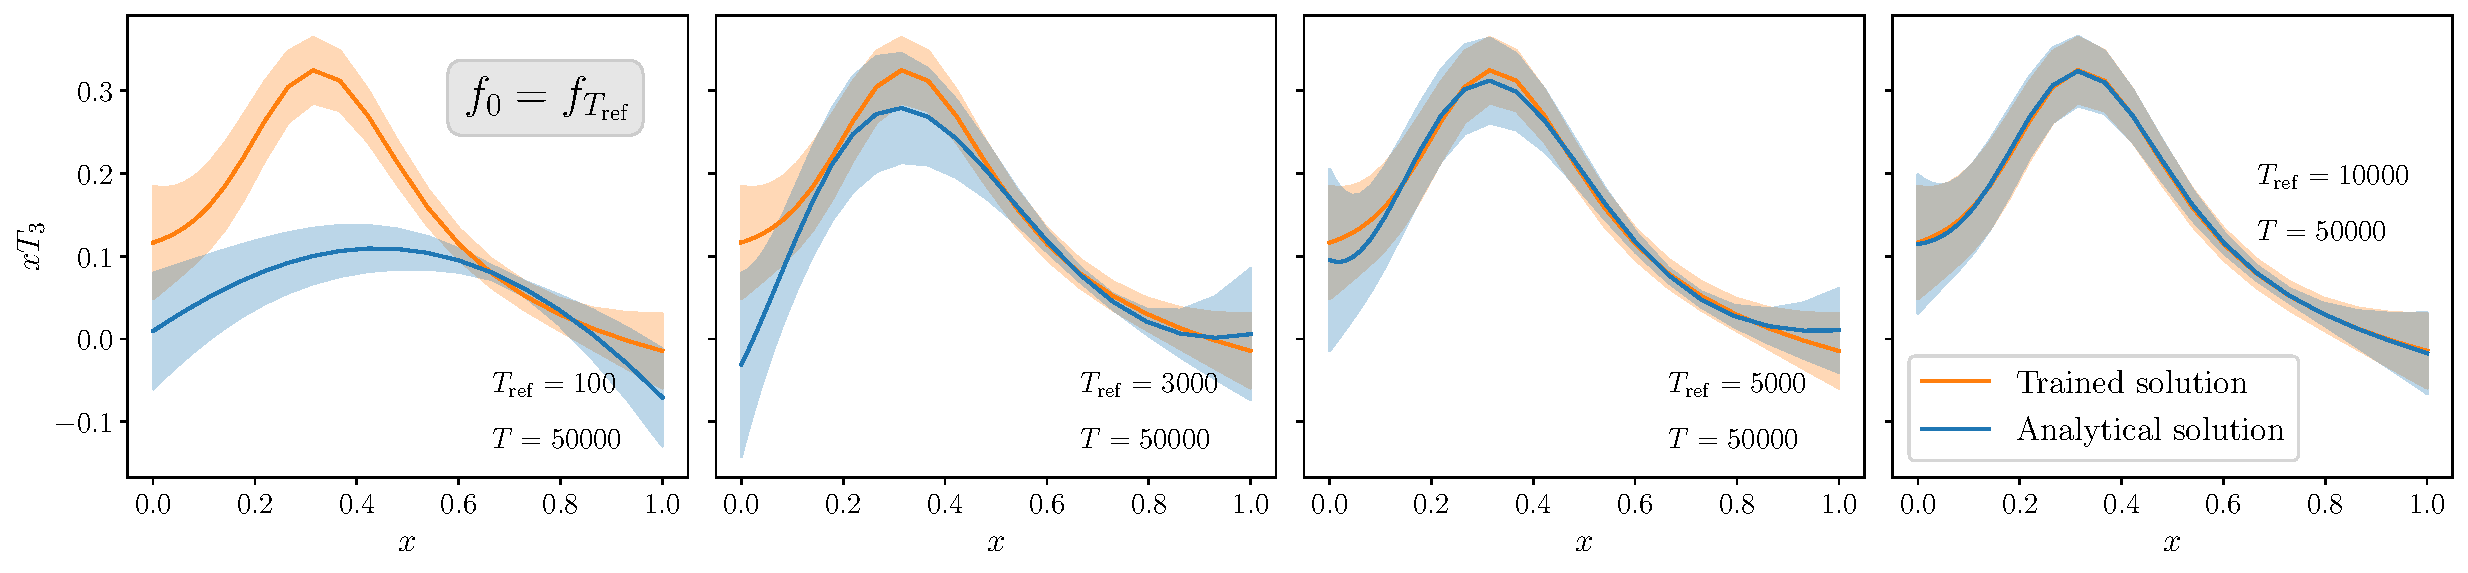
\includegraphics[width=0.9\textwidth]{section_4/evolution_vs_trained_ftref_L2.pdf} 
  \caption{Comparison of the trained and analytical evolution at the end of
  training. Each panel corresponds to a different frozen NTK, whereby the
  analytical solution is computed starting from $f_{T_{\rm Ref}}$. The orange
  curve represents the final trained function after 50000 iterations of GD, and
  is the same across panels. Error bands represent one-sigma uncertainties
  across replicas. L2 data is used.}
  \label{fig:OnsetLazyL2}
\end{figure}
% =================================================
The solution in Eq.~\eqref{eq:AnalyticSol} is the main result of this section.
It shows that the training process can be described as the sum of a linear
transformation of the initial fields $f_{0,\alpha}$, and a linear transformation
of the data $Y_I$. The two transformations depend on the flow time $t$ and are
given by the evolution operators $U(t)$ and $V(t)$. Fig.~\ref{fig:OnsetLazyL2}
compares the analytical solution with the trained function at the end of
training, for different choices of the frozen NTK. The evolution time $T$ used
in the analytical solution is the difference between the total training time and
$T_{\rm ref}$. Central value and uncertainty bands are obtained by computing the
analytical solution for each replicas of the initial condition and frozen NTK.
\footnote{
  If not stated otherwise, in this section central values and uncertainties are
  always computed as ensemble averages across replicas.
}
The figures agree with the expectation; the closer $T_{\rm ref}$ is to the
onset of the lazy regime, the better the agreement between the analytical
solution and the trained function.

A complementary perspective is provided in Fig.~\ref{fig:FrefDecompositionL2},
where the analytical solution is decomposed into the two contributions from $U$
and $V$. In each panel, the initial condition $f_{T_{\rm ref}}$ is evolved
analytically for different training times by keeping the frozen NTK fixed. We
see that as training proceeds, the contribution from $U$ is progressively
suppressed, in accordance with the observation made above. On the other hand,
the contribution from $V$ grows and becomes dominant at later epochs, indicating
that the trained function is mostly determined by the data, rather than the
previous condition of the network. We also observe that such behaviour happens
quite rapidly, as a consequence of the fact the time scales in the analytical solution are
determined by the inverse of the eigenvalues of $H^\perp$, and latter 
are typically large.
% Decomposition L2 ================================
\begin{figure}[ht]
    \centering
    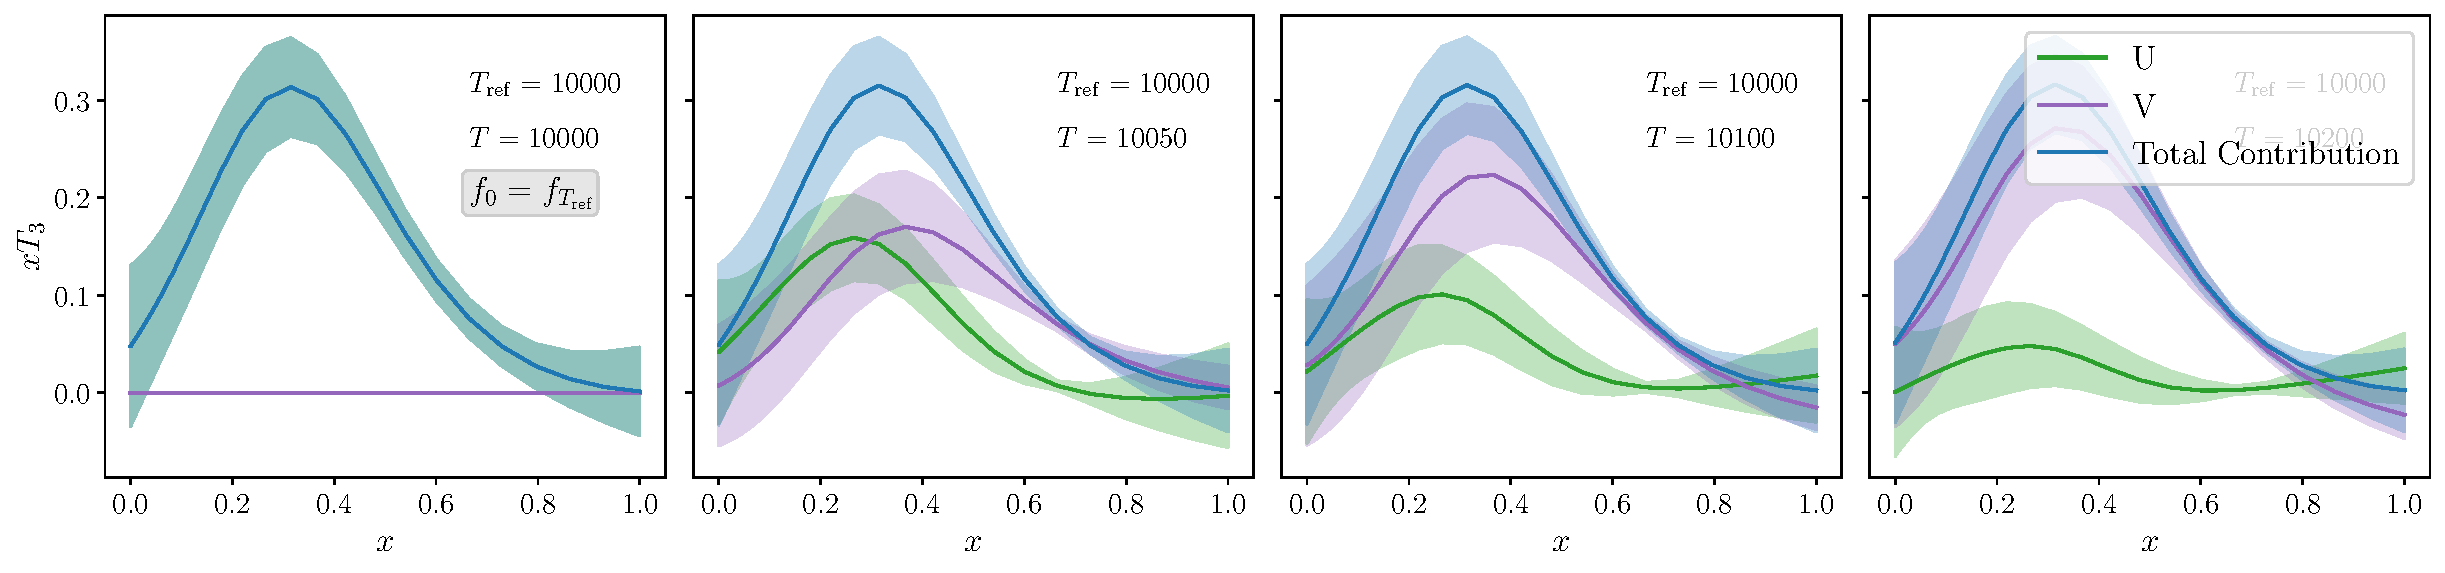
\includegraphics[width=0.9\textwidth]{section_4/u_v_decomposition_L2.pdf} 
    \caption{Decomposition of the analytical solution into the two contributions
    from $U$ and $V$ at different training times. The frozen NTK is fixed across
    panels, and corresponds to the one at $T_{\rm ref} = 10000$. The initial
    condition is always $f_{T_{\rm ref}}$. As in Fig.~\ref{fig:OnsetLazyL2}, L2 data
    is used.}
    \label{fig:FrefDecompositionL2}
  \end{figure}
  % =================================================
  
  
The analytical solution in Eq.~\eqref{eq:AnalyticSol} sheds a new light onto the
behaviour of the numerical training of a neural network. Given these results, it
is natural to ask whether the information encoded in the NTK alone can drive
training beyond its original initial condition, \ie\ whether the analytical
solution can be used to perform kernel learning. We address this question in the
following section.

\subsection{Lazy Training as Kernel Learning}
\label{sec:NTKKernelLearning}

The results shown in Sec.~\ref{sec:Lazy} and Sec.~\ref{sec:NTKDuringTraining}
support the idea that the NTK is capable to encode in its eigenvectors 
the physical features learned
during training. We now probe this idea further by employing the analytical
solution in Eq.~\eqref{eq:AnalyticSol} \textit{\`a la} kernel learning, \ie\ by
applying it to an initial condition that represents our prior. In the following,
we choose the initial condition to be an ensemble of networks at initialisation
as in Fig.~\ref{fig:prior}, whose architecture is the same as the one used in
the training. This represents our prior assumption on the space of functions,
which is then updated using the data and the NTK frozen at $T_{\rm ref}$.

\subsubsection{Convergence of the Analytical Solution}
% Grid plot with L2 ================================
\begin{figure}[t]
  \centering
  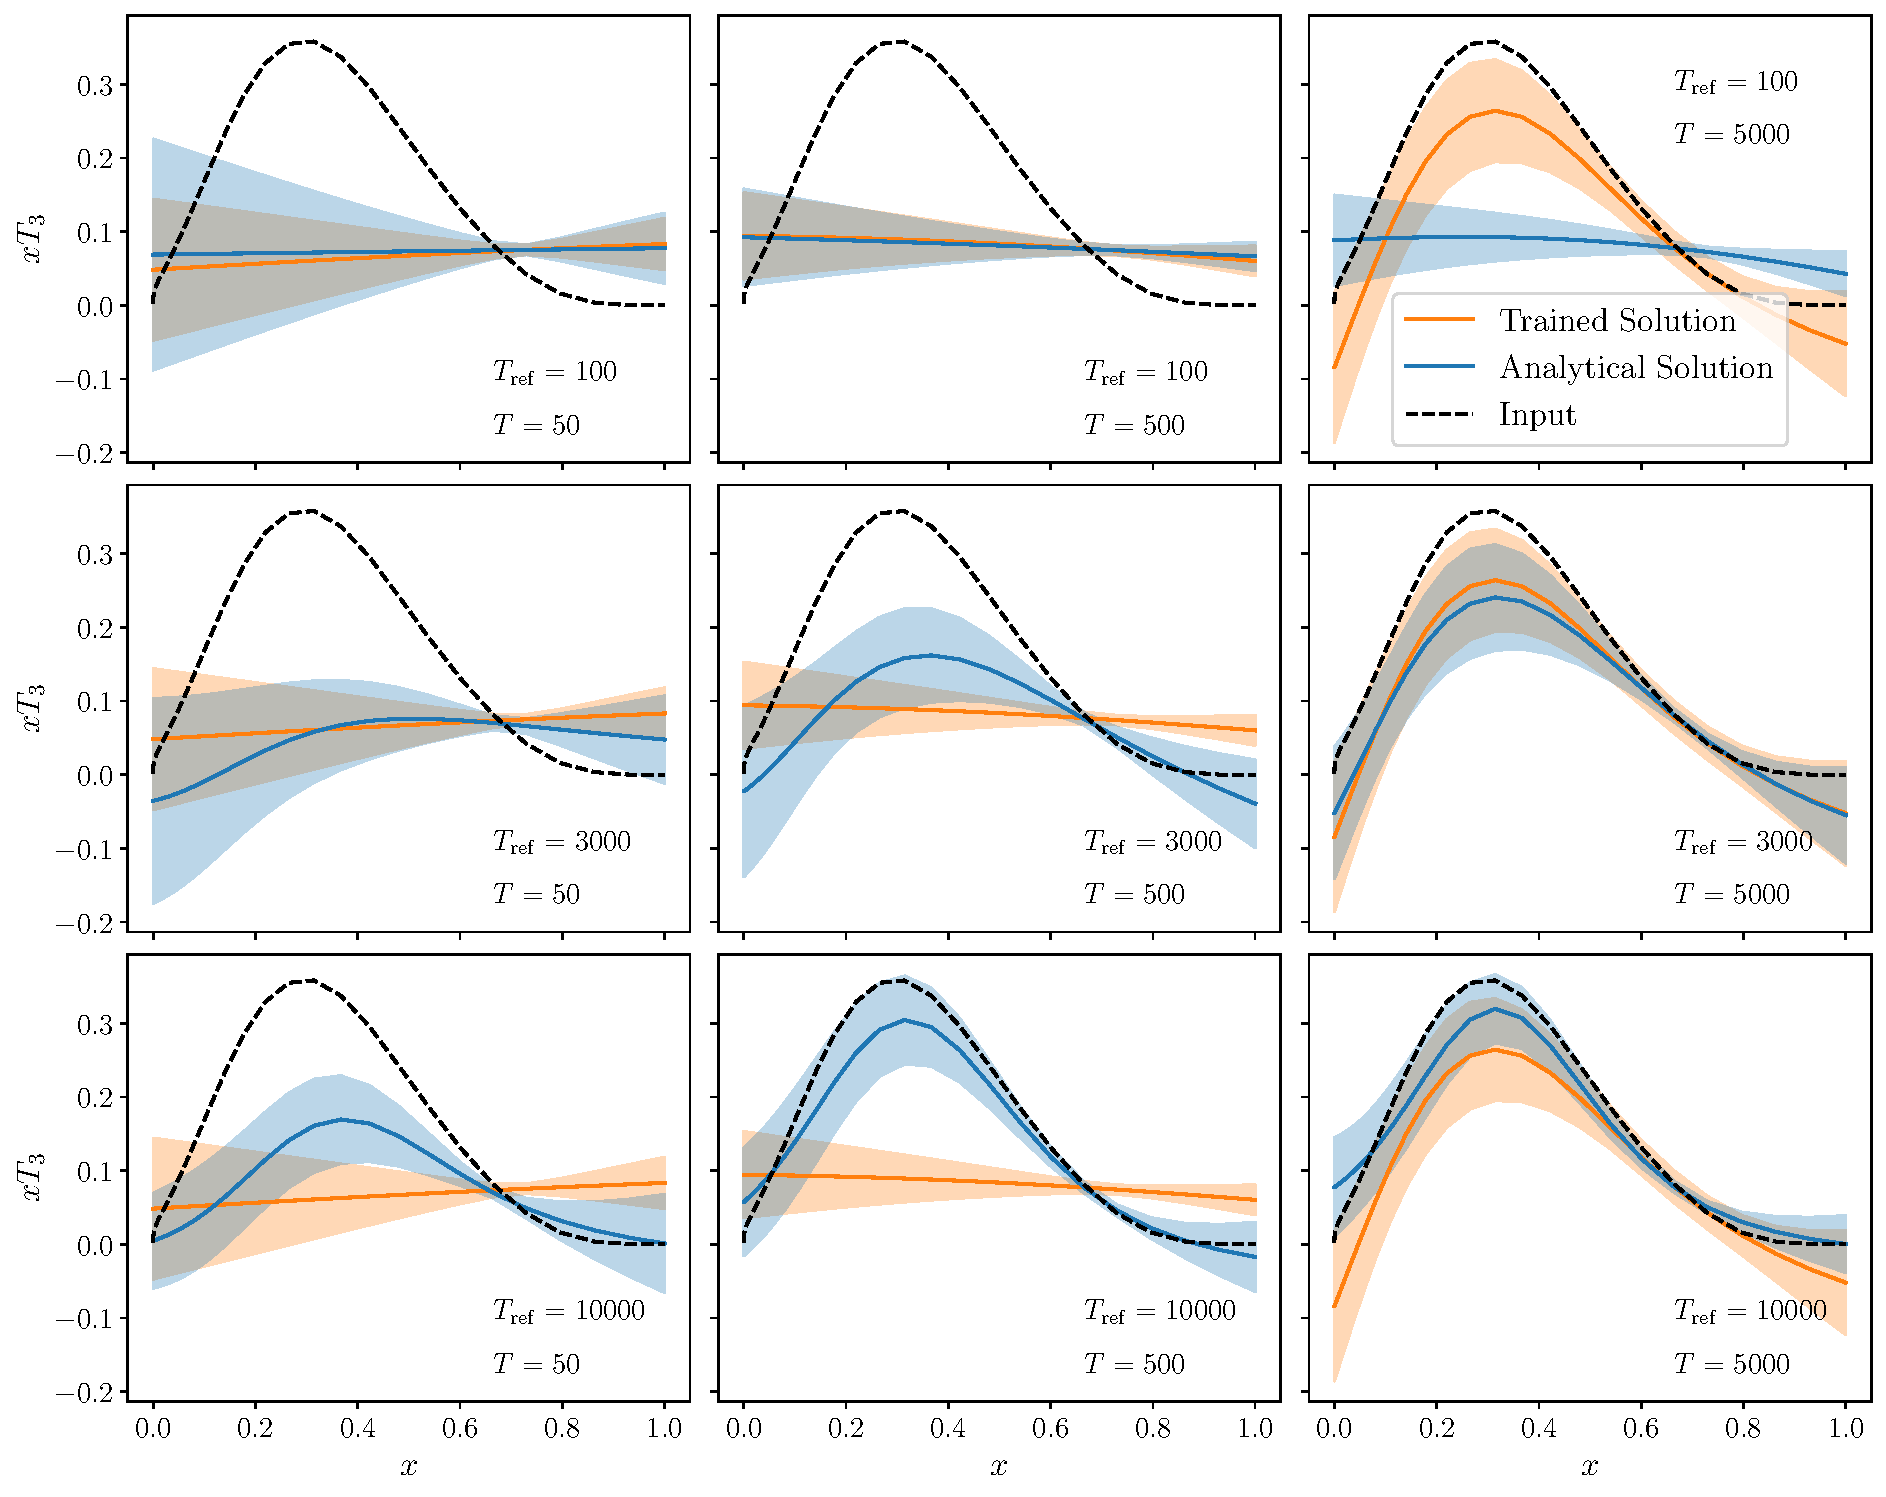
\includegraphics[width=0.9\textwidth]{section_4/evolution_f0_vs_trained_grid_L2.pdf} 
  \caption{Comparison of the trained (orange) and analytical (blue) evolution
  starting from an ensemble of networks at initialisation as the initial
  condition. Each row corresponds to a different frozen NTK, while the columns
  represent different training times. L2 data is used.}
  \label{fig:EvolutionGridF0L2}
\end{figure}
% =================================================
We start by comparing the analytical solution (AS), obtained using an ensemble
of networks at initialisation as the initial condition, with the trained
solution (TS), obtained after training a neural network from a different initial
condition. This comparison is shown in Fig.~\ref{fig:EvolutionGridF0L2} for L2
data, where the rows in the grid correspond to different frozen NTKs, while the
columns represent numerical and analytical evolution after $T=50, 500$ and 5000
epochs. These results deserve a few comments.

The first observation is that the NTK at early stages of training is not able to
drive the prior towards the true function, as shown in the first and, though
less dramatically, in the second row of Fig.~\ref{fig:EvolutionGridF0L2}. This
is expected, as we extensively discussed in Sec.~\ref{sec:NTKDuringTraining},
since at early stages the NTK has not yet aligned its internal representation
with the data.

More significantly, we observe a significant discrepancy between the AS and the
TS even at $T=5000$. This can be explained as follows. At the beginning of
training, there is clearly no difference between AS and TS since both represent
the neural network output at initialisation (Sec.~\ref{sec:Init}), with
variations due only to different initialisation seeds. During early training
stages, AS and TS differ as expected. Indeed, the analytical solution is
computed using the frozen NTK at $T_{\rm ref}$, while the trained solution
evolves with an NTK that is still changing as shown in Sect.~\ref{sec:Training}.
Crucially, if the NTK at $T_{\rm ref}$ has already learned from the data and
aligned with the solution, the AS converges faster to the target, while the TS
requires additional epochs before evolving in the correct direction.

\subsubsection{Central Value and Covariance of the Trained Fields}
\label{sec:CentralAndCovariance}

The analytical solution in Eq.~\eqref{eq:AnalyticSol} is inherently stochastic,
since the frozen NTK at $T_{\rm ref}$ is actually obtained from an ensemble of
networks. As a consequence, the operators $U(t)$ and $V(t)$ are both random
variables. We can then characterize the distribution of the analytical solution
using the mean and variance across the ensemble, as shown in
Eq.~\eqref{eq:ReplicaEnsemble}. The central value of the trained field is thus
defined as
\begin{align}
    \label{eq:MeanValAtT}
    \bar{f}_{t,\alpha} = \mathbb{E}\left[f_{t,\alpha}\right]
        = \mathbb{E}\left[U(t)_{\alpha\alpha'} f_{0,\alpha'}\right]
            + \mathbb{E}\left[V(t)_{\alpha I} Y_I\right] \, .
\end{align}
More interestingly, we can also compute the covariance matrix of the trained
fields at any time $T$,
\begin{align}
    \cov[f_t,f_t^T]
        &= \mathbb{E}\left[U(t) f_0 f_0^T U(t)^T\right] 
            - \mathbb{E}\left[U(t) f_0\right] \mathbb{E}\left[f_0^T U(t)^T\right]  \nonumber \\
        &\quad + \mathbb{E}\left[U(t) f_0 Y^T V(t)^T\right] 
            - \mathbb{E}\left[U(t) f_0\right] \mathbb{E}\left[Y^T V(t)^T\right] \nonumber \\
        &\quad + \mathbb{E}\left[V(t) Y f_0^T U(t)^T\right]
            - \mathbb{E}\left[V(t) Y\right] \mathbb{E}\left[f_0^T U(t)^T\right] \nonumber \\
    \label{eq:CovAtT}
        &\quad + \mathbb{E}\left[V(t) Y Y^T V(t)^T\right]
            - \mathbb{E}\left[V(t) Y\right] \mathbb{E}\left[Y^T V(t)^T\right] \, .
\end{align}
Note that the first and the fourth lines above yield symmetric matrices, while
the third line is just the transpose of the second, thereby ensuring that the
whole covariance matrix is the sum of three symmetric matrices and therefore is
symmetric, 
\begin{align}
    \label{eq:SumOfCovariances}
    \cov[f_t,f_t^T] = C_t^{(00)} + C_t^{(0Y)} + C_t^{(YY)}\, ,
\end{align}
where
\begin{align}
    \label{eq:C00term}
    C_t^{(00)} 
        &= \mathbb{E}\left[U(t) f_0 f_0^T U(t)^T\right] 
        - \mathbb{E}\left[U(t) f_0\right] \mathbb{E}\left[f_0^T U(t)^T\right]\, ,\\
    C_t^{(0Y)}
        &= \mathbb{E}\left[U(t) f_0 Y^T V(t)^T\right] 
        - \mathbb{E}\left[U(t) f_0\right] \mathbb{E}\left[Y^T V(t)^T\right] \nonumber \\
        \label{eq:C0Yterm}
        &\quad + \mathbb{E}\left[V(t) Y f_0^T U(t)^T\right]
            - \mathbb{E}\left[V(t) Y\right] \mathbb{E}\left[f_0^T U(t)^T\right] \, ,\\
    C_t^{(YY)}
        &= \mathbb{E}\left[V(t) Y Y^T V(t)^T\right]
        - \mathbb{E}\left[V(t) Y\right] \mathbb{E}\left[Y^T V(t)^T\right]\, .
\end{align}
Eq.~\eqref{eq:SumOfCovariances} shows that the factorisation between the
contribution from the initial condition and the one from the data holds also at
the level of the covariance matrix. Indeed, $C_t^{(00)}$ quantifies the
contribution to the covariance matrix that is purely due to the fluctuations of
the initial condition, while $C_t^{(YY)}$ quantifies the contribution that is
purely due to the statistical fluctuations of the data. The mixed term
$C_t^{(0Y)}$ accounts for the correlations between the two sources of
uncertainty.


\paragraph{Connection with Linear Methods}
% ===================================
\begin{figure}[t!]
  \centering
  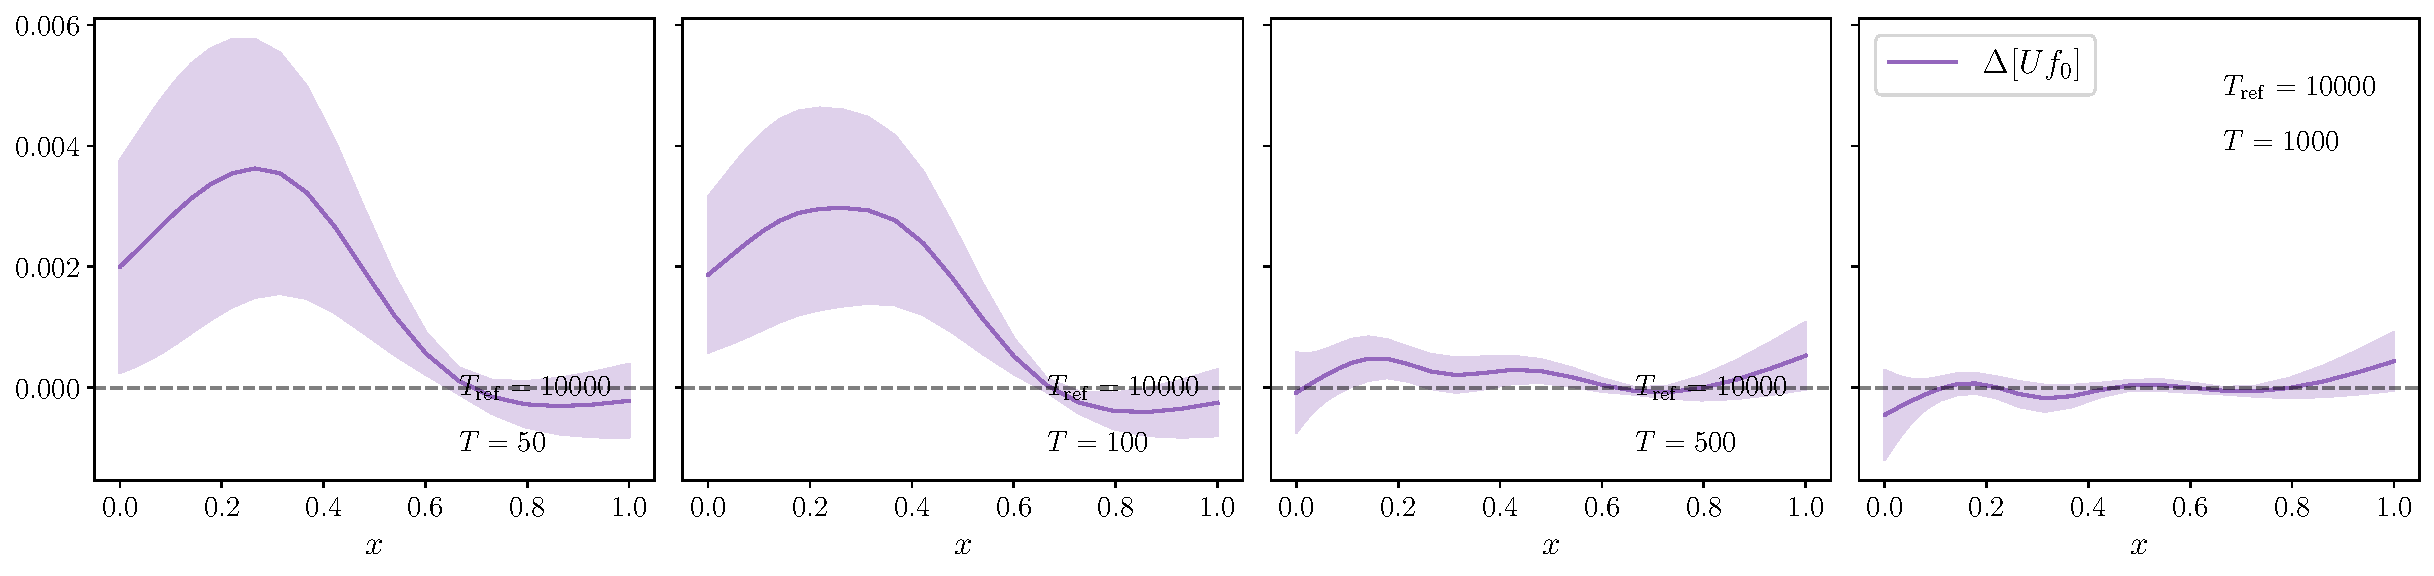
\includegraphics[width=0.95\textwidth]{section_4/delta_bootstrap_L2_U.pdf}
  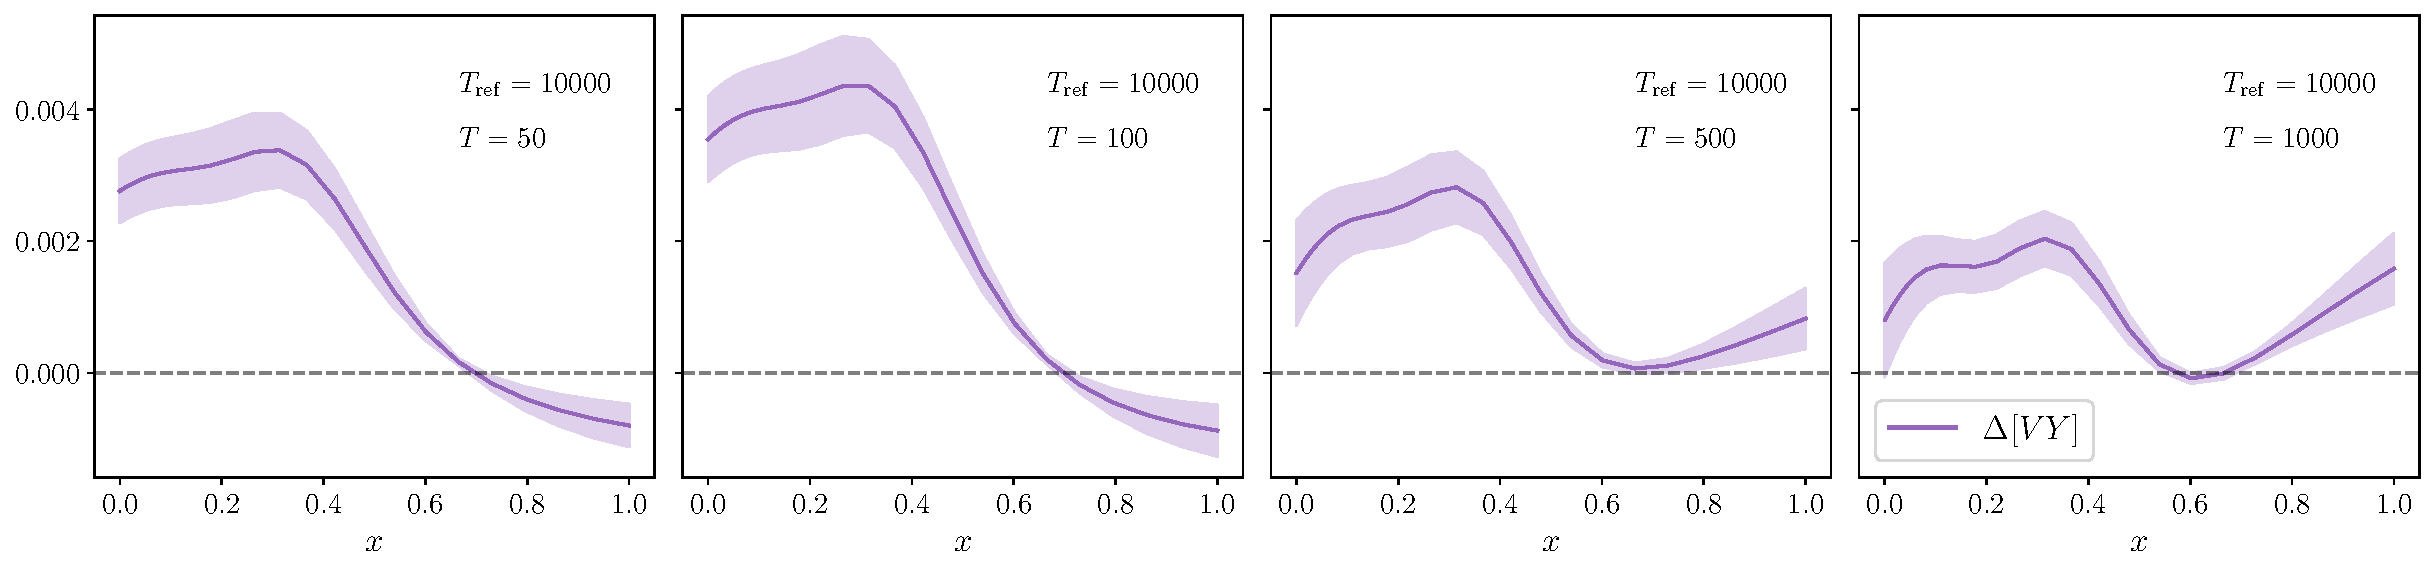
\includegraphics[width=0.95\textwidth]{section_4/delta_bootstrap_L2_V.pdf}
  \caption{Behaviour of $\Delta [U(t)f_0]$ and $\Delta [V(t)Y]$, as defined in
  Eqs.~\eqref{eq:DeltaExpValUtF0} and~\eqref{eq:DeltaExpValVtY}, as functions
  of the training
  time. The operators $U(T)$ and $V(T)$ are constructed by taking the 
  NTK at $T_{\rm ref} = 10000$, which is fixed across panels. The uncertainties are extracted
  from the bootstrap ensemble as discussed in the text.}
    \label{fig:xT3_exp_val}
\end{figure}
% ===================================

We can consider a simplifying limit of Eq.~\eqref{eq:MeanValAtT}, where the
initial condition $f_0$ and the data $Y$ are statistically independent
from the respective
evolution operators $U(t)$ and $V(t)$. Note that the first term on the right-hand
side of Eq.~\eqref{eq:MeanValAtT} can only be non-zero because of the
correlations between $U(t)$ and $f_0$. In the absence of such correlations, the
first term would be given by the product of the expectation values and therefore
would vanish if $f_0$ is an ensemble of networks at initialisation. Under these
assumptions, we have
\begin{align}
    \label{eq:MeanUt}
    \bar{U}(t)
        &= \mathbb{E}\left[U(t)\right]\, , \\
    \label{eq:MeanVt}
    \bar{V}(t)
        &= \mathbb{E}\left[V(t)\right]\, ,
\end{align}
and
\begin{equation}
    \label{eq:MeanValAtTNoCorr}
    \bar{f}_{t,\alpha} = \bar{U}(t)_{\alpha\alpha'} \bar{f}_{0,\alpha'}
        + \bar{V}(t)_{\alpha I} Y_I = \bar{V}(t)_{\alpha I} Y_I \, .
\end{equation}
The second term in Eq.~\eqref{eq:MeanValAtT}, or equivalently
Eq.~\eqref{eq:MeanValAtTNoCorr}, explicitly shows the contribution of each data
point to the central value of the trained fields at each value of $x_{\alpha}$.
It is worthwhile remarking that in this limit, the central value from the set of
trained networks is a linear combination of the data points, with coefficients
given by the evolution operator $V(t)_{\alpha I}$.

In the absence of general theorems, we verify this assumption empirically.
From the ensemble of replicas, we generate bootstrap samples and compute the
following two estimators,
\begin{align}
    \label{eq:DeltaExpValUtF0}
    \Delta[U(f)f_0] &= \mathbb{E}\left[U(t) f_{0}\right] 
      - \mathbb{E}\left[U(t) \right] \mathbb{E}\left[f_{0}\right]\, , \\
    \label{eq:DeltaExpValVtY}
    \Delta[V(f)Y] &= \mathbb{E}\left[U(t) Y\right] 
      - \mathbb{E}\left[V(t) \right] \mathbb{E}\left[Y\right]\, .
\end{align}
for different training times, using the same frozen NTK and L2 data. The results
are shown in Fig.~\ref{fig:xT3_exp_val} for the $U$ (upper panel) and $V$ (lower
panel) contributions. The error bands are computed using bootstrap error. By
inspecting the figures, we see two distinct patterns emerging. For the operator 
$U$, $\Delta[U f_0]$ is different from zero for small training times, and thus the
correlations between $U(t)$ and $f_0$ are non-negligible. However, as training
proceeds, the $\Delta[U f_0]$ becomes compatible with zero within the error bars, 
suggesting that the correlations are progressively suppressed.
The case of the $V$ operator is even more striking, as $\Delta[V Y]$ is clearly
non-negligible across all training times, although it also shows a decreasing trend as
training proceeds. This suggests that the correlations between $V(t)$ and $Y$
cannot be neglected. 

In conclusion, we note that Eq.~\eqref{eq:MeanValAtTNoCorr} resembles the structure
of a linear method, like \eg\ Backus-Gilbert or Gaussian Processes. We believe
that this observation, as well as the results shown in
Fig.~\ref{fig:xT3_exp_val}, deserve further investigations, which we leave for
future work.

\paragraph{Error decomposition}
% ===================================
\begin{figure}[t!]
  \centering
  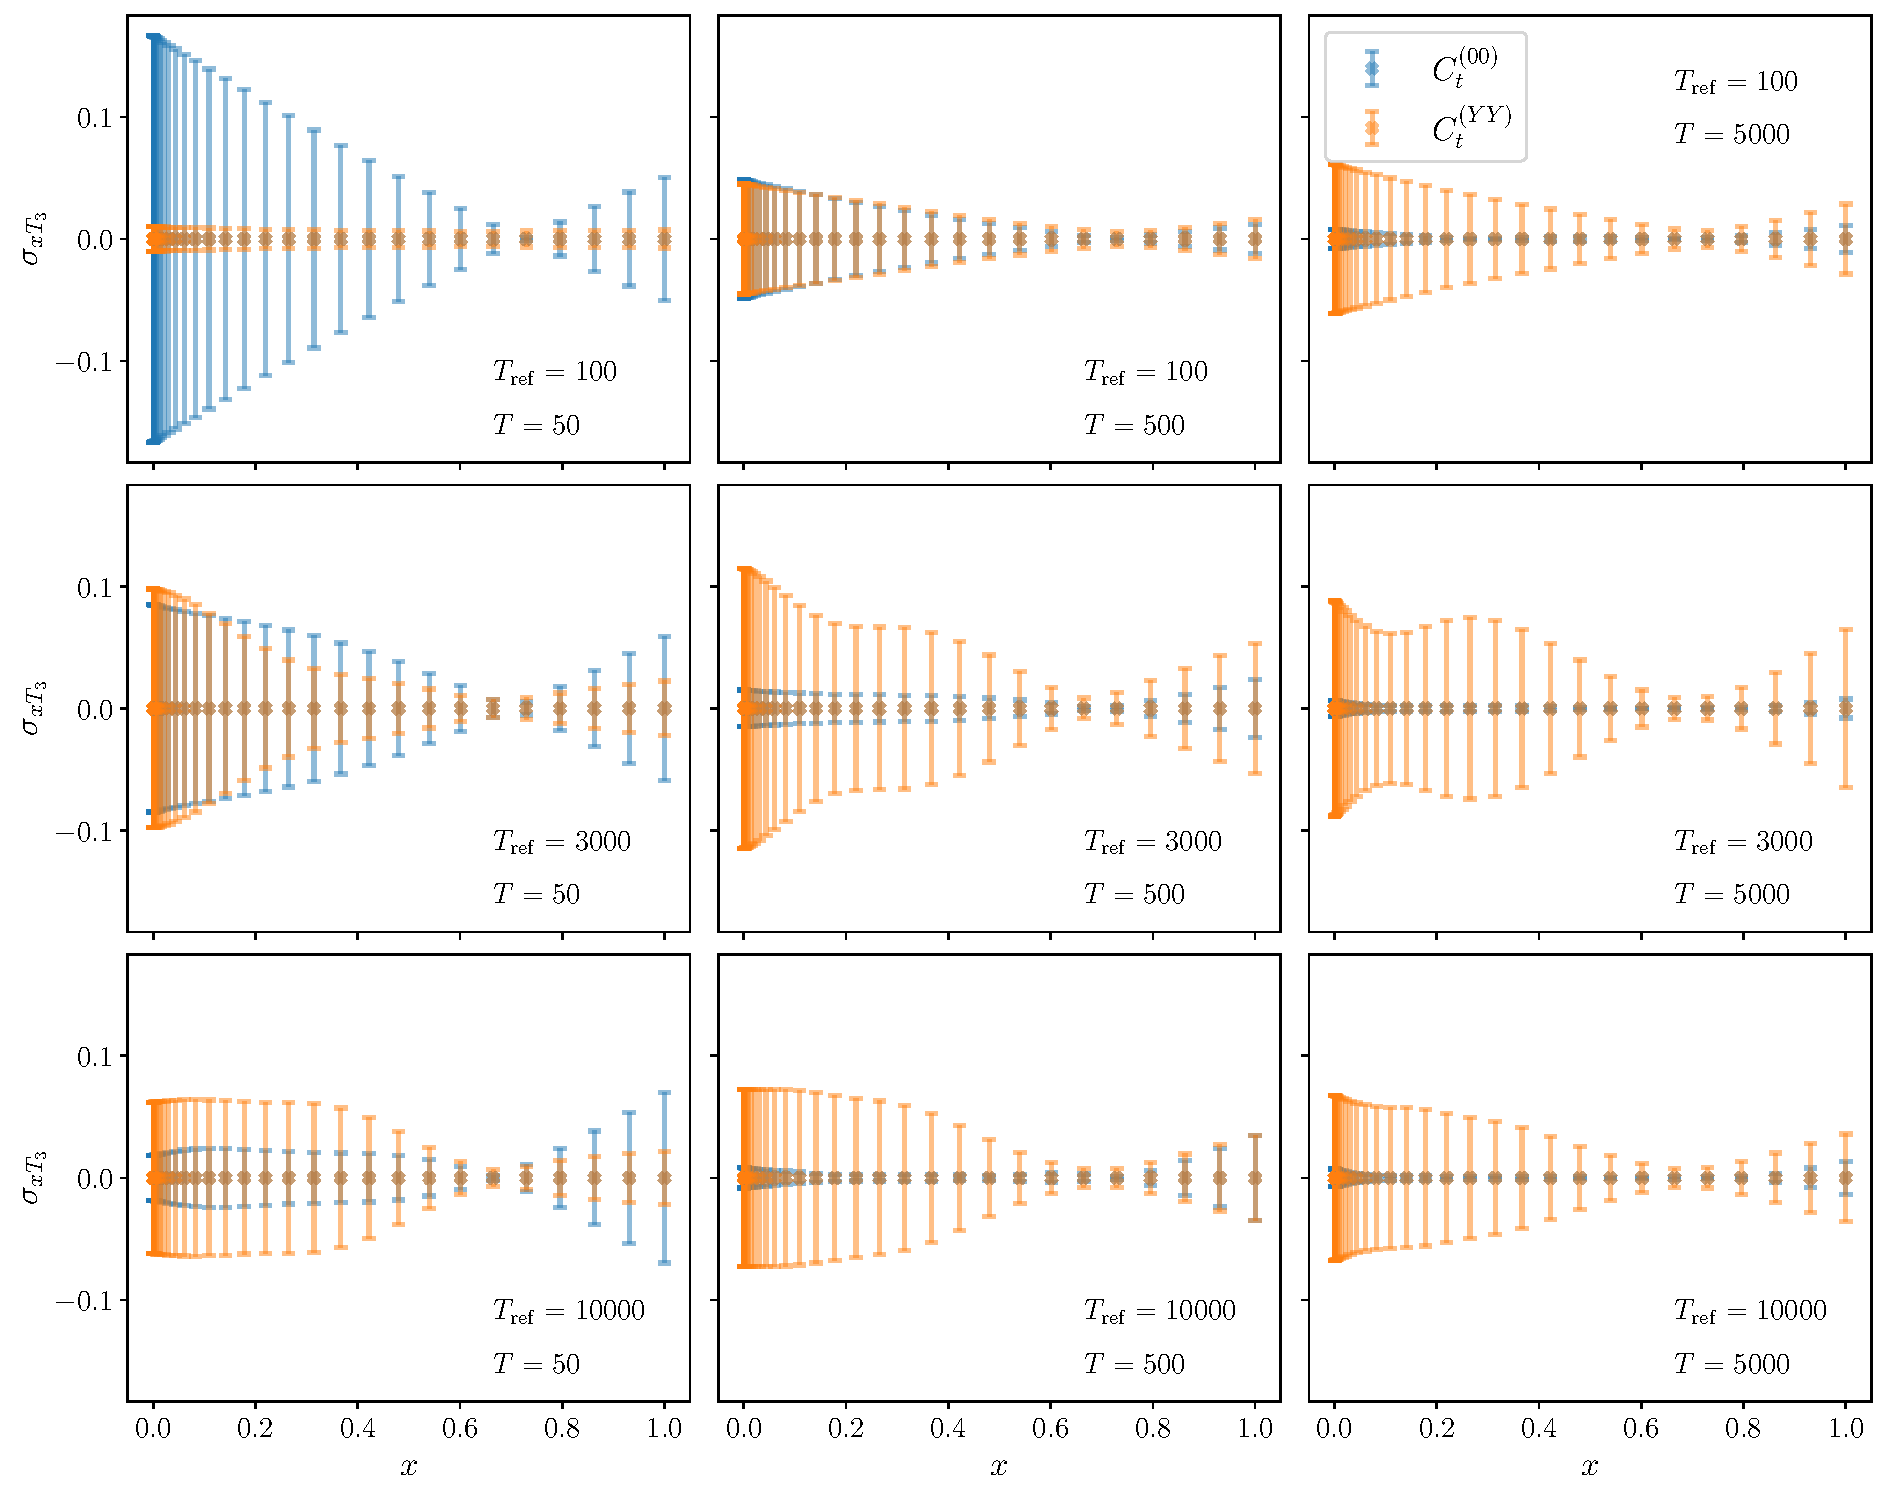
\includegraphics[width=0.9\textwidth]{section_4/error_buddget_L2.pdf}
  \caption{}
  \label{fig:ErrorBudgetL2}
\end{figure}
% ===================================
The analytical expression for the covariance matrix,
Eq.~\eqref{eq:SumOfCovariances}, allows us to monitor the relative size of the
three contributions as training proceeds. For a properly trained ensemble of 
networks, the covariance of the trained fields should be
dominated by the statistical error on the data. We show the diagonal entries of
the decomposition of the error budget in Fig.~\ref{fig:ErrorBudgetL2}, for
different frozen NTKs (rows) and different training epochs (columns), using L2
data as before. In general, we observe that towards the end of the training 
process the
contribution from the data $C_t^{(YY)}$ (orange band) becomes dominant with
respect to the contribution coming from the initial condition $C_t^{(00)}$ (blue
band). We also see that the suppression of the initial condition is more severe
and happens earlier when the frozen NTK is taken at later stages of training.
These findings ensure that the quoted error on the PDFs is actually dominated by
the statistical error on the data, and not by the fluctuations of the initial
fields. This is a crucial point, since it guarantees that the error bars computed
from the ensemble of
trained PDFs is not biased by the choice of prior that is made by selecting a
given architecture, activation function, and probability distribution for the
biases and weights at initialisation.

\subsubsection{Crosschecks using L0 data}
\label{sec:AnalyticalChecks}

The analytical solution enables rigorous validation of our implementation 
through crosschecks with L0 data, where we have complete control over 
the data generation process. In this case, the realization of the dataset is 
completely determined by the input PDFs
\begin{equation}
    \label{eq:DataL0NoIndices}
    Y = \FKtab \fin\, .
\end{equation}
Note that using L0 data only affects the second term in
Eq.~\ref{eq:AnalyticSol}.\footnote{To be more precise, since the analytical
solution requires the NTK to be frozen at a certain epoch $T_{\rm ref}$, the
NTK will depend on the data used in the training.} We can then rewrite
the combined term in Eq.~\eqref{eq:DataCorrectedInference} as follows
\begin{align}
  \label{eq:TrainingOnLevelZero}
  \check{U}^\perp(t) f_0 + V(t) Y 
    &= \mathcal{M}(t)\, \FKtabT C_{Y}^{-1} \FKtab\, 
      \left[\fin - f_{0}^\parallel\right]\, .
\end{align}
The subtraction taking place in the square brackets of
Eq.~\eqref{eq:TrainingOnLevelZero} suggests us that the effective function that
the neural network actually sees is not the input function $\fin$ used to
generate the data, but rather the difference between $\fin$ and the component of
the initial function $f_0$ that lies in the subspace spanned by the kernel of
the NTK, \ie\ $f_0^\parallel$. In other words, the parallel component
$f_0^\parallel$, which we remind does not evolve during the analytic training,
acts as a constant ``bias'' in the training process, shifting the effective
input function that the neural network sees. Of course the actual magnitude of
this irreducible noise depends both on how $f_0$ and the kernel of the NTK are
distributed over the ensemble. We will come to this point soon.

Note that the observation above remains true even in the limit of infinite
training. This can be shown using 
\begin{align}
    \label{eq:LevelZeroClosureInfiniteTraining}
    \lim_{t\to\infty} V(t) Y = \finperp + \mathcal{M}_{\infty} M \finpar\, ,
\end{align}
which shows that the $V$ component of the trained solution reproduces exactly the
component of the PDF that lies in  the subspace orthogonal to the kernel of
$\Theta$. We compare the asymptotic behaviour of $V(t) Y$ and $\finperp$ in
Fig.~\ref{fig:InfiniteTimeVterm}.

\begin{figure}[t]
  \centering
  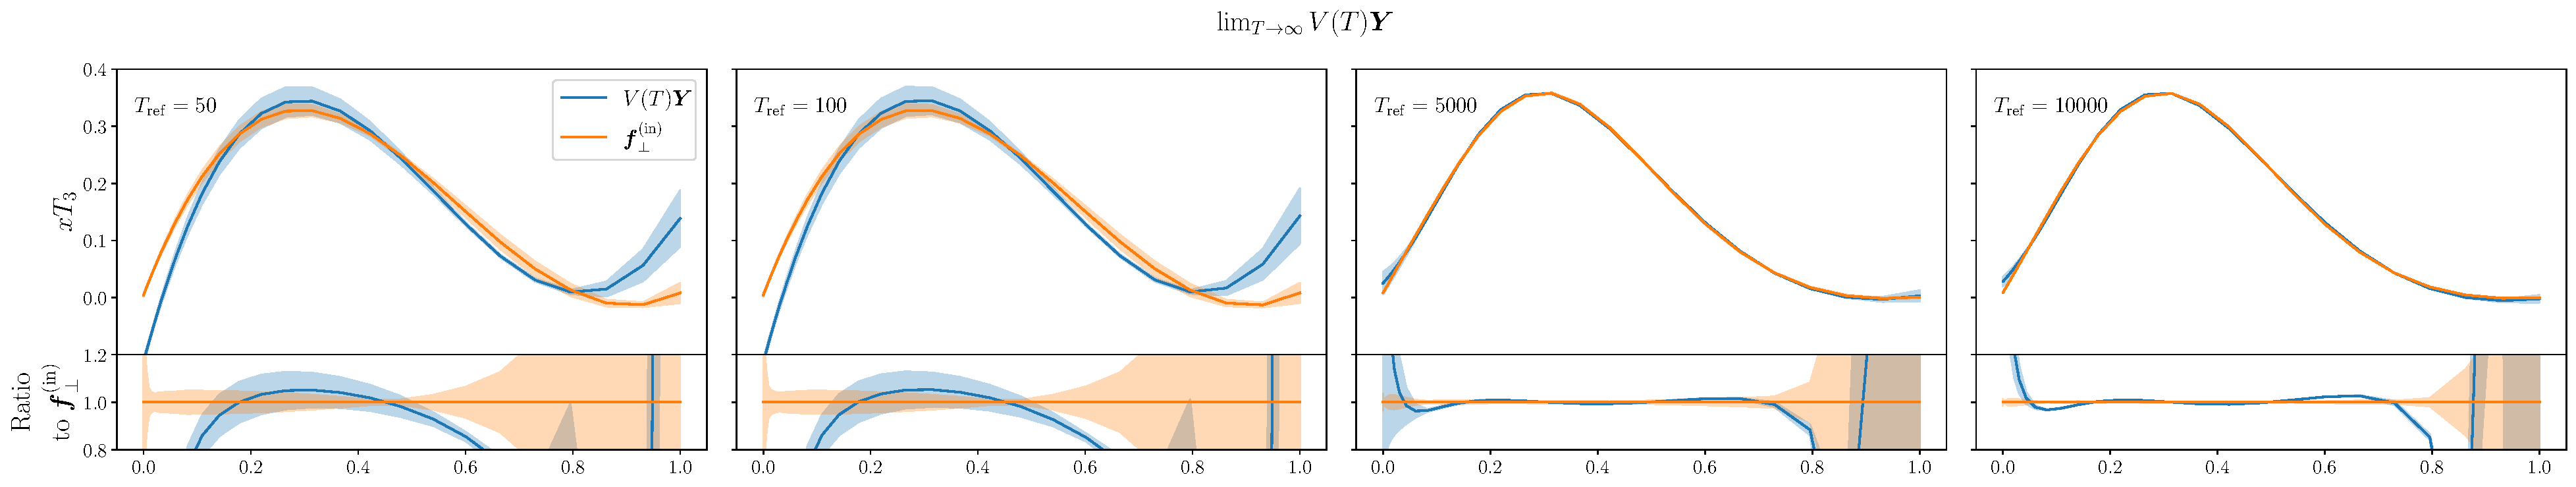
\includegraphics[width=\textwidth]{section_4/vy_inf_L0.pdf}  
  \caption{Test the $t\to\infty$ limit of the L0 training for different frozen
  NTK. The orange curve represents the projection of the input function $\fin$
  onto the subspace orthogonal to the kernel of the NTK at $T_{\rm ref}$, \ie\
  $\finperp$. The blue curve represents the contribution of the operator $V$,
  computed with the NTK at $T_{\rm ref}$, in the limit of infinite training
  time.}
  \label{fig:InfiniteTimeVterm}
\end{figure}

The second term in the square bracket on the right-hand side of
Eq.~\eqref{eq:TrainingOnLevelZero} is the contribution from the parallel
component at initialisation that does not evolve in the training process. Given
that $f_0$ is almost normally distributed around zero, that term does not
contribute to the central value of the fitted PDF, \ie\ to the average of the
trained solution over replicas. The time evolution of 
\begin{align}
  \label{eq:AverageLevelZeroUcheck}
  \mathbb{E}\left[\mathcal{M}(t)\, \FKtabT C_{Y}^{-1} \FKtab\, 
    f_{0}^\parallel\right]\, ,
\end{align}
is shown in Fig.~\ref{fig:AverageLevelZeroUcheck}.
\begin{figure}[h!]
  \centering
  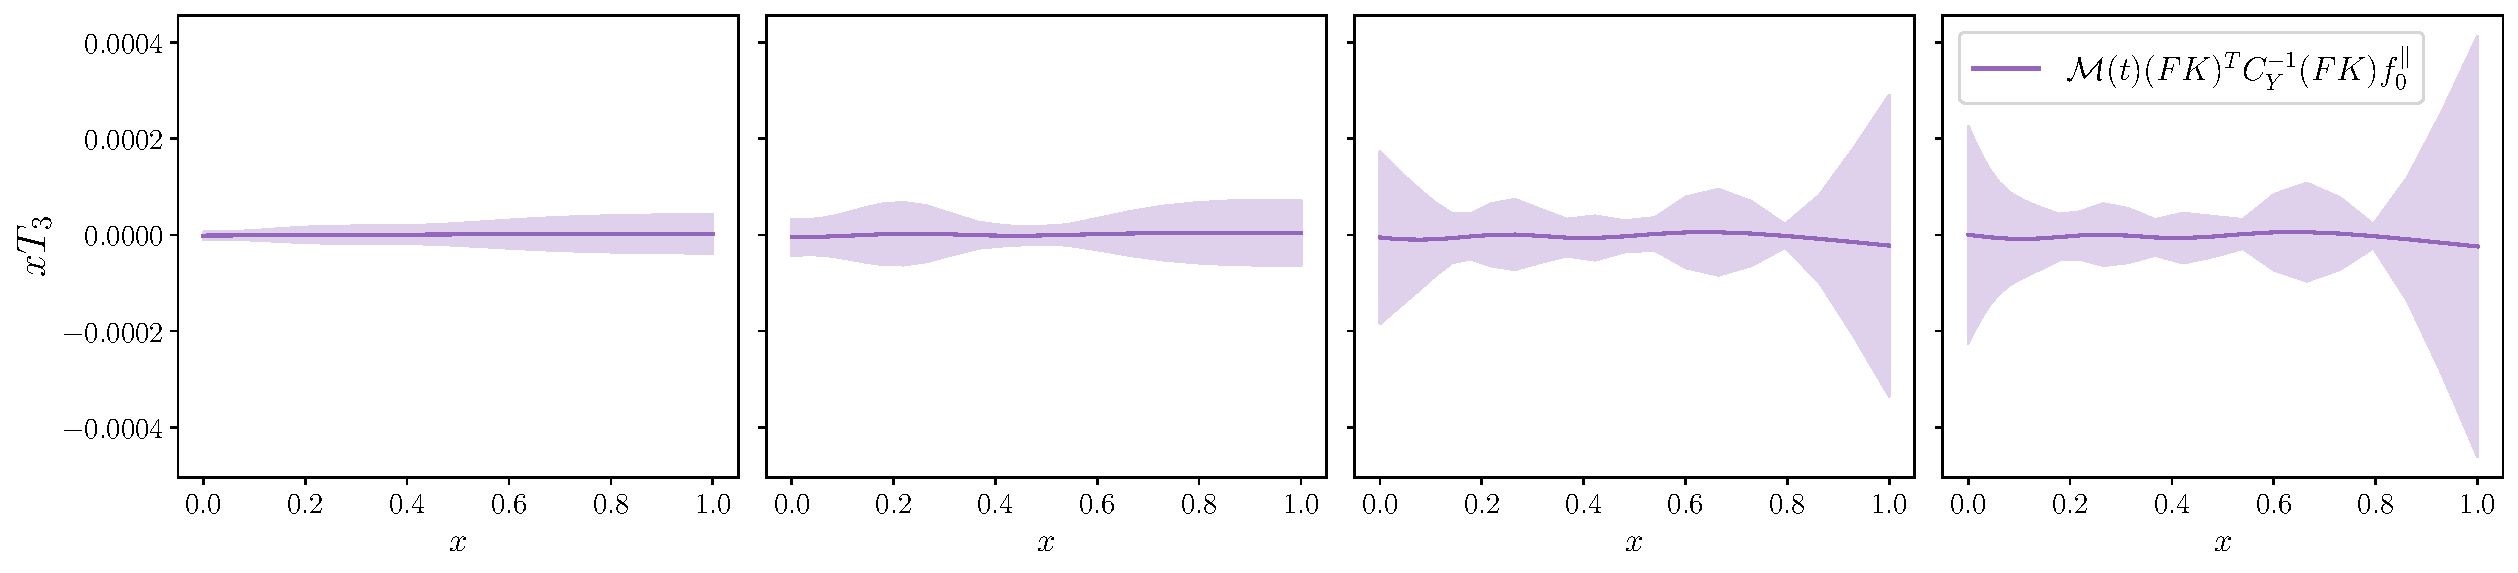
\includegraphics[width=0.95\textwidth]{section_4/Mcal_M_fpar_L2_linear.pdf} 
  \caption{Test of the average of the parallel contribution for different
  epochs. The reference epoch at which the frozen NTK is chosen is $T_{\rm ref}
  = 10000$. L2 data is used in the plot.}
  \label{fig:AverageLevelZeroUcheck}
\end{figure}

\subsubsection{Infinite Training Time}
In the limit of infinite training time, the evolution operators $U(t)$ and
$V(t)$ simplify and yield an elegant interpretation of the minimum of the cost
function. For large training times, we have
\begin{align}
    \label{eq:UhatInfty}
    \hat{U}^\perp_{\infty, \alpha\alpha'}
        &= \lim_{t\to\infty}\hat{U}^\perp(t)_{\alpha\alpha'} = 0\, \\
    \label{eq:MOperatorInfty}
    \mathcal{M}_{\infty, \alpha\alpha'} 
        &= \lim_{t\to\infty}\mathcal{M}(t)_{\alpha\alpha'} = \sum_{k,k'\in\perp} \sqrt{\lambda^{(k)}} z^{(k)}_\alpha 
        \left[\sideset{}{'}\sum_{i} w^{(i)}_{k} \frac{1}{h^{(i)}}\, 
        w^{(i)}_{k'}\right] z^{(k')}_{\alpha'} \sqrt{\lambda^{(k')}}\, ,
\end{align}
and explicit expressions for $\check{U}^\perp_{\infty}$ and $V_{\infty}$ are
obtained from $\mathcal{M}_{\infty}$. The term in the square bracket in
Eq.~\eqref{eq:MOperatorInfty} is the spectral decomposition of the pseudoinverse
of $H^\perp$ in $d_\perp$ orthogonal subspace. So, the operator
$\mathcal{M}_{\infty}$ acts as follow on a field $f_{\alpha}$:
\begin{enumerate}
    \item The term on the right of the square bracket computes the coordinate
    $f_k$ introduced in Eq.~\eqref{eq:OrthogonalComponents}. The $f_k$ are a set
    of coordinates for the component $f^\perp$ of the field that evolves during
    training, 
    \begin{align}
        \label{eq:RightOfTheBracket}
        f^\perp = \sum_{k\in\perp} \sqrt{\lambda^{(k)}} f_k\, z^{(k)}\,  .
    \end{align}
    \item The term in the square bracket applies the pseudoinverse to the
    coordinates $f_k$, 
    \begin{align}
        \label{eq:ApplyPseudoInv}
        f'_k = \left(H^\perp\right)^+_{kk'} f_{k'}\, .
    \end{align}
    \item The final term on the left of the square bracket reconstructs the full
    field corresponding to the modified $f'_{k}$,
    \begin{align}
        \label{eq:LeftOfTheBracket}
        f^{'\perp} = \sum_{k\in\perp} \sqrt{\lambda^{(k)}} f'_{k}\, z^{(k)}\, .
    \end{align}
    
\end{enumerate}

As discussed at the end of Sect.~\ref{sec:Lazy} it is convenient to combine the
contributions of $\check{U}^\perp_{\infty}$ and $V_{\infty}$,
\begin{align}
    \label{eq:DataCorrectedInferenceAtInfty}
    \check{U}^{\perp}_{\infty} f_{0} + V_{\infty} Y 
        = \mathcal{M}_{\infty}\; \FKtabT C_Y^{-1} \left[Y - \FKtab f_{0}^{\parallel}\right]\, .
\end{align}
The contribution to the observables from the parallel components of $f$ does not
change during training, therefore that contribution is subtracted from the data
and the orthogonal components of $f$ are adjusted to minimize the $\chi^2$ of
the corrected data. The minimum of the $\chi^2$ in the orthogonal subspace is
found applying $\mathcal{M}_{\infty}$, \ie\ by projecting in the orthogonal
subspace, applying the pseudoinverse and finally recompute the full field as
detailed above.


\FloatBarrier